% Jeffrey Hong Spring 2019
\begin{blocksection}
\question A \textit{bipartite} graph has the property that its vertices can be divided into two non-overlapping subsets \textit{A} and \textit{B} such that every edge in the graph has one vertex in set \textit{A} and one vertex in set \textit{B}. There are no edges between two vertices that are both in set \textit{A} or two vertices that are both in set \textit{B}.

The graph below is bipartite, since it can be partitioned into subsets \{1, 3\} and \{2, 4\}.
\begin{center}
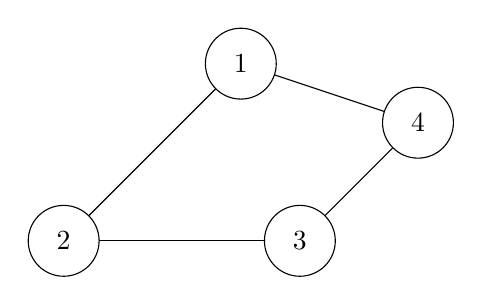
\begin{tikzpicture}[scale=0.15]
\tikzstyle{every node}+=[inner sep=0pt]
\draw (25,-15) circle (3);
\draw (25,-15) node {$1$};
\draw (10,-30) circle (3);
\draw (10,-30) node {$2$};
\draw (30,-30) circle (3);
\draw (30,-30) node {$3$};
\draw (40,-20) circle (3);
\draw (40,-20) node {$4$};
\draw (22.88,-17.12) -- (12.12,-27.88);
\draw (37.15,-19.05) -- (27.85,-15.95);
\draw (37.88,-22.12) -- (32.12,-27.88);
\draw (13,-30) -- (27,-30);
\end{tikzpicture}
\end{center}

Alternatively, adding an edge between vertices 1 and 3 creates a graph that is not bipartite.
\begin{center}
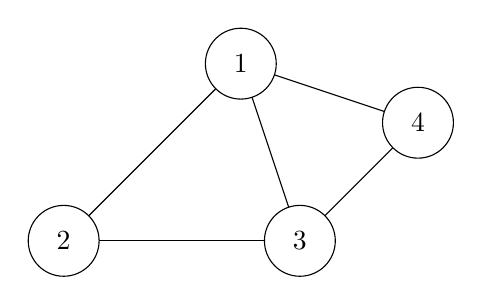
\begin{tikzpicture}[scale=0.15]
\tikzstyle{every node}+=[inner sep=0pt]
\draw (25,-15) circle (3);
\draw (25,-15) node {$1$};
\draw (10,-30) circle (3);
\draw (10,-30) node {$2$};
\draw (30,-30) circle (3);
\draw (30,-30) node {$3$};
\draw (40,-20) circle (3);
\draw (40,-20) node {$4$};
\draw (22.88,-17.12) -- (12.12,-27.88);
\draw (37.15,-19.05) -- (27.85,-15.95);
\draw (37.88,-22.12) -- (32.12,-27.88);
\draw (13,-30) -- (27,-30);
\draw (25.95,-17.85) -- (29.05,-27.15);
\end{tikzpicture}
\end{center}

Describe a graph traversal that returns \textit{True} if a given undirected graph is bipartite and \textit{False} if it is not.

\begin{solution}
Either DFS or BFS can be used. Starting at an arbitrary vertex, mark (or color) all vertices that are one edge away, then continue and do not mark (color differently) all vertices that are two edges away, etc. If no neighbor of a vertex has the opposite marking or color, then the graph is bipartite.
Since marking each vertex and checking its neighbors is linear and happens in the graph traversal process, the runtime is then the same as DFS/BFS, which is $O(|V| + |E|)$.
\end{solution}
\end{blocksection}